\par\medskip\noindent\begin{minipage}{\linewidth}

\centering\small
\captionof{table}{All descriptive validation-MSE targets in the new regression tasks. Each entry is the first epoch at which the validation tuning profile reaches the stated fraction of the common initial validation MSE. Every method has 13 optimizer settings; finite prefixes of later-stopped runs are eligible. A dash denotes an unreached target by epoch 2000. These are validation-selected iteration profiles, not wall-clock benchmarks or single executable training trajectories.}
\label{tab:new-task-hitting}
\begin{tabular}{lrrrrr}
\toprule Task & Relative target & AdamW & SGD-M & Balance & QO\\\midrule
SDF / SIREN & $10^{-1}$ & 2 & 2 & 2 & 2\\
SDF / SIREN & $10^{-2}$ & 11 & 28 & 16 & 17\\
SDF / SIREN & $10^{-3}$ & 157 & 1350 & 403 & 403\\
SDF / SIREN & $10^{-4}$ & \textemdash & \textemdash & 1183 & 1142\\
SDF / SIREN & $10^{-6}$ & \textemdash & \textemdash & \textemdash & \textemdash\\
Burgers / DeepONet & $10^{-1}$ & 73 & 292 & 47 & 47\\
Burgers / DeepONet & $10^{-2}$ & 297 & \textemdash & 651 & 584\\
Burgers / DeepONet & $10^{-3}$ & \textemdash & \textemdash & \textemdash & \textemdash\\
Burgers / DeepONet & $10^{-4}$ & \textemdash & \textemdash & \textemdash & \textemdash\\
Burgers / DeepONet & $10^{-6}$ & \textemdash & \textemdash & \textemdash & \textemdash\\
Matrix completion & $10^{-1}$ & 16 & 25 & 19 & 19\\
Matrix completion & $10^{-2}$ & 43 & 57 & 48 & 45\\
Matrix completion & $10^{-3}$ & 67 & 502 & 71 & 69\\
Matrix completion & $10^{-4}$ & 138 & \textemdash & 117 & 107\\
Matrix completion & $10^{-6}$ & 215 & \textemdash & 162 & 150\\
\bottomrule
\end{tabular}

\end{minipage}\par\medskip
\par\medskip\noindent\begin{minipage}{\linewidth}

\centering
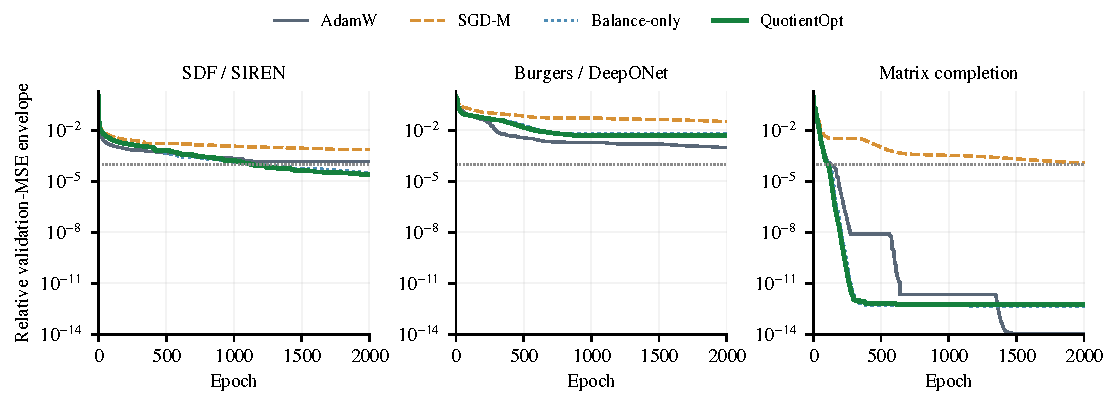
\includegraphics[width=.99\linewidth]{figures/new_task_convergence_profiles.pdf}
\captionof{figure}{Validation tuning envelopes from every completed regression-task block. At each epoch the envelope takes the best finite validation checkpoint among all 13 settings and earlier epochs, including prefixes of later-stopped trials. It is a descriptive equal-budget tuning profile, not one optimizer trajectory. The horizontal line is the $10^{-4}$ relative-MSE target; Table~\ref{tab:new-task-hitting} retains all five targets. Values below $10^{-14}$ are drawn at the plotting floor for legibility.}
\label{fig:new-task-convergence}

\end{minipage}\par\medskip
